\begin{figure}[tb]
	\centering
	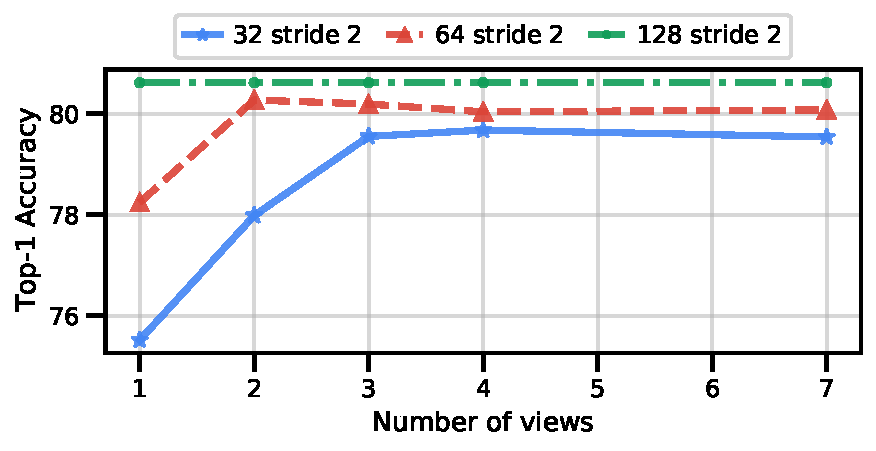
\includegraphics[width=0.95\linewidth]{figures/ablation/views_accuracy_frames.pdf}
	\caption{
		The effect of varying the number of frames input to the network and increasing the number of tokens proportionally.
		We use ViViT-L/16x2 Factorised Encoder on Kinetics 400.
		A Kinetics video contains 250 frames (10 seconds sampled at 25 fps) and the accuracy for each model saturates once the number of equidistant temporal views is sufficient to ``see'' the whole video clip.
		Observe how models processing more frames (and thus more tokens) achieve higher single- and multi-view accuracy.
	}
	\label{fig:ablation_num_frames}
	\vspace{-\baselineskip}
\end{figure}